\documentclass{article}
\usepackage[utf8]{inputenc}

\title{Assignment of Operational Statistics for SAR Imagery}
\author{Nan Lin\\ \texttt{19171213734} }
\date{October 2019}

\usepackage{natbib}
\usepackage{graphicx}
\usepackage{subfigure}

\begin{document}

\maketitle

\section{Introduction}
In the assignment, I selected a sample from urban from the image shown in Fig. 3.4. And I analyzed the data with G$^0$ distribution. 

\section{The Multiplicative Models}
In this course, we mainly studied the multiplicative model, which is one of the myriad methods for building stochastic descriptions for sar data. The reason for choosing this model is that it can make sar image data expressible and easy to handle.\\
We learned three models that can fit the data from SAR image, which are Gamma distribution,K distribution and G$^0$ distribution.\\
The density of Gamma distribution uses the $\Gamma$ function, which has the following properties.
\begin{eqnarray}
\Gamma(x+1)=x\Gamma(x)\\
\Gamma(n)=(n-1)!  
\end{eqnarray}
The density of Gamma distribution is the following.
\begin{eqnarray}
f(z;L;\sigma^2)=\frac{L^L}{\sigma^{2L}\Gamma(L)}exp(\frac{-Lz}{\sigma^2})
\end{eqnarray}
The density of K distribution is the following.

\begin{eqnarray}
f(z;\alpha,\lambda,L)=\frac{2L\lambda}{\Gamma(\alpha)\Gamma(L)}(Lz\lambda)^(\frac{\alpha+L}{2}-1)K_{\alpha-L}(2\sqrt{Lz\lambda})
\end{eqnarray}

\begin{eqnarray}
K_{v}(z)=\int_{0}^\infty{exp(-z)\cosh(vt)dt}
\end{eqnarray}
The density of G0 distribution is the following.
\begin{eqnarray}
f(z;\alpha,\gamma,L)=\frac{L^L\Gamma(L-\alpha)}{\gamma^\alpha\Gamma(L)\Gamma(-\alpha)}\frac{z^(L-1)}{(\gamma+Lz)^(L-\alpha)}
\end{eqnarray}
I used ggplot to plot the densities of the above three distributions.The results are showed in Figure 1. 
\begin{figure}[htbp]
\centering
\subfigure[Gamma distribution]{
\begin{minipage}[t]{0.33\linewidth}
\centering
\includegraphics[width=1.5in]{gamma.png}
%\caption{fig1}
\end{minipage}%
}%
\subfigure[K distribution]{
\begin{minipage}[t]{0.33\linewidth}
\centering
\includegraphics[width=1.5in]{G0.png}
%\caption{fig2}
\end{minipage}
}%
\subfigure[G$^0$ distribution]{
\begin{minipage}[t]{0.33\linewidth}
\centering
\includegraphics[width=1.5in]{K.png}
%\caption{fig2}
\end{minipage}
}%
\centering
\caption{The densities of Gamma,K,G$^0$ distributions}
\end{figure}
\section{Data Analysis}
The content shown in Figure 2(a) is Fig 3.4 in the assignment. I select some data of urban from the lower left corner, as shown in Figure 2(b). The histogram is obtained by using the hist function, as shown in Figure 3(a). When selecting the model, I found that the shape of the curve of the g0 distribution is most consistent with the gray image of the data, and using a single distribution to fit the data does not obtain good results. So, in order to better fit the data, I select some data from it and use three G$^0$ distribution with different parameters to fit, and get better results, as shown in Figure 3(b).\\

\begin{figure}[htbp]
\centering
\subfigure[sar image]{
\begin{minipage}[t]{1\linewidth}
\centering
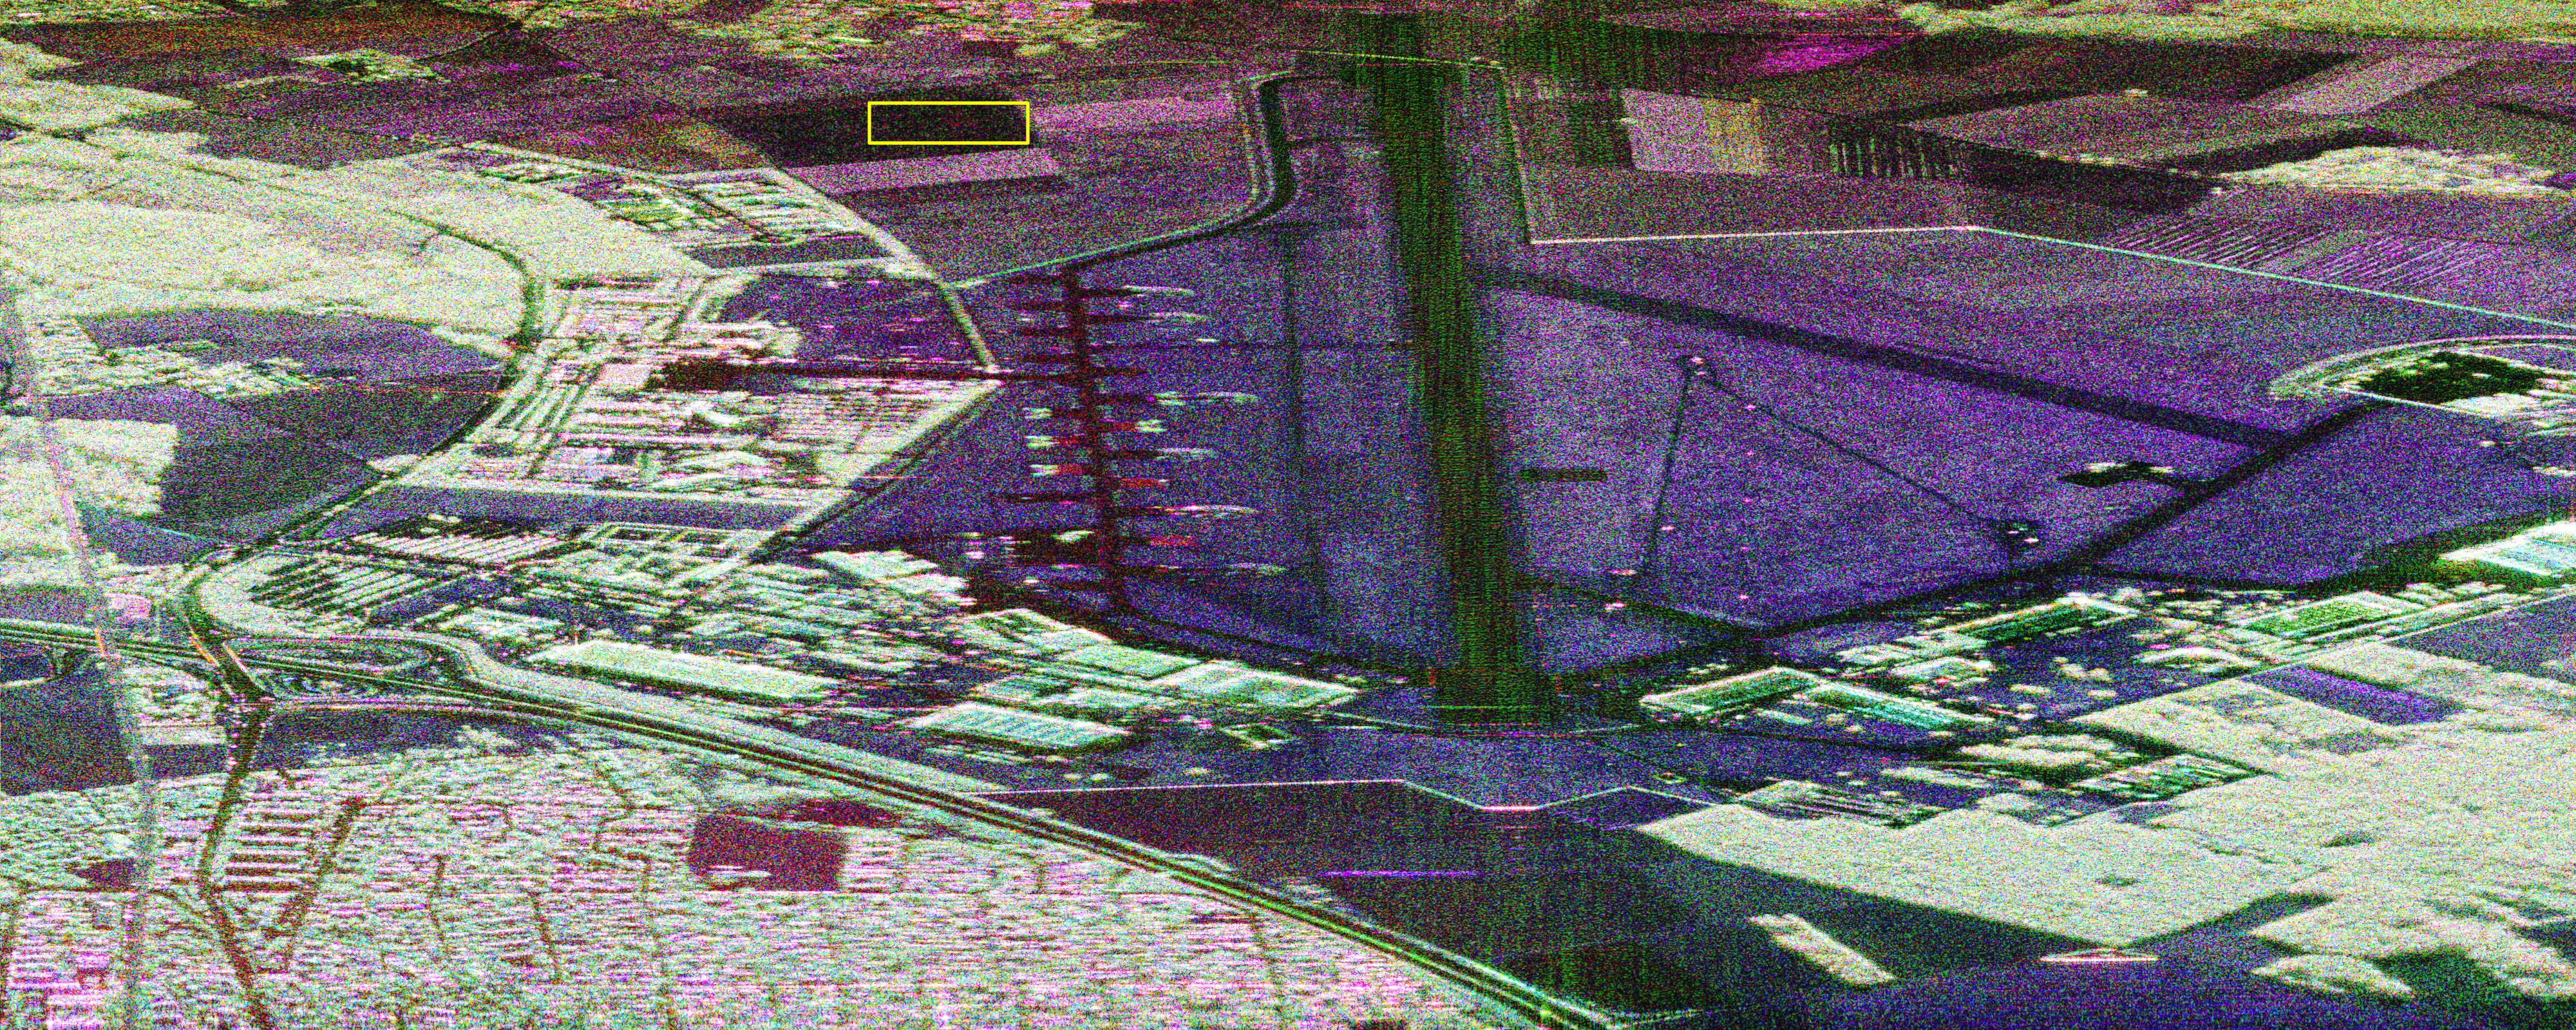
\includegraphics[width=4in]{sar.png}
%\caption{fig1}
\end{minipage}%
}%

\subfigure[urban image]{
\begin{minipage}[t]{1\linewidth}
\centering
\includegraphics[width=1in]{sar-urban.png}
%\caption{fig2}
\end{minipage}
}%
\centering
\caption{SAR image and captured urban image}
\end{figure}
\begin{figure}[ht]
\subfigure[histogram]{
\begin{minipage}[t]{0.5\linewidth}
\centering
\includegraphics[width=2in]{hist.png}
%\caption{Histogram}
\end{minipage}%
}%
\subfigure[results]{
\begin{minipage}[t]{0.5\linewidth}
\centering
\includegraphics[width=2in]{results.png}
%\caption{Results}
\end{minipage}
}%
\caption{Histogram and fitting results}
\end{figure}
\end{document}
